\documentclass[12pt]{article}
% LaTeX packages and global styles
% used packages in the template
% import your package here 
\usepackage[utf8]{inputenc}
\usepackage{multicol}
\usepackage{xcolor}
\usepackage{subfigure}
\usepackage{siunitx}
%
\usepackage[utf8]{inputenc}
\usepackage{graphicx}
\usepackage{titlesec}
\usepackage[bookmarks,breaklinks,colorlinks=true,allcolors=blue]{hyperref}
\usepackage{listings}
\usepackage{inconsolata}
\usepackage{float}
\usepackage{eso-pic}
\usepackage[framemethod=tikz]{mdframed}

\usepackage[square,numbers]{natbib}
\AtBeginDocument{
  \renewcommand{\bibsection}{\chapter{\bibname}}
} % Bibliography in numbered chapter

\usepackage{geometry}
\usepackage{amsmath}
\usepackage{parskip}
\usepackage[official]{eurosym}
\setlength {\marginparwidth }{2cm} 
\usepackage{todonotes}
\usepackage{csquotes}

\usepackage{rotating}
\usepackage{lmodern}
\usepackage{setspace}
\usepackage{pdfpages}
\usepackage{svg}

% style sheet for the thesis
% Chapter and section title format
\titleformat{\section}[block]{\normalfont\huge\bfseries}{\thesection.}{.5em}{\Huge}[{}]
% \titlespacing*{\chapter}{0pt}{-19pt}{25pt}
% \titleformat{\section}[block]{\normalfont\Large\bfseries}{\thesection.}{.5em}{\Large}


\usepackage{listings}
\usepackage{xcolor}

\definecolor{codegreen}{rgb}{0,0.6,0}
\definecolor{codegray}{rgb}{0.5,0.5,0.5}
\definecolor{codepurple}{rgb}{0.58,0,0.82}
\definecolor{backcolour}{rgb}{0.95,0.95,0.92}

\lstdefinestyle{mystyle}{
    backgroundcolor=\color{backcolour},   
    commentstyle=\color{codegreen},
    keywordstyle=\color{magenta},
    numberstyle=\tiny\color{codegray},
    stringstyle=\color{codepurple},
    basicstyle=\ttfamily\footnotesize,
    breakatwhitespace=false,         
    breaklines=true,                 
    captionpos=b,                    
    keepspaces=true,                 
    numbers=left,                    
    numbersep=5pt,                  
    showspaces=false,                
    showstringspaces=false,
    showtabs=false,                  
    tabsize=2
}
% code formatting with listing
\lstset{
  style=mystyle
}

% Margins
\geometry{
    a4paper,
    margin=2.75cm
}

% Index depth limit
\setcounter{tocdepth}{2}

% Paragraph Indentation
\setlength{\parindent}{1cm}

\renewcommand{\lstlistingname}{Code extraction}
\renewcommand*{\lstlistlistingname}{Code Excerpts Index}

\definecolor{US_red}{cmyk}{0, 1, 0.65, 0.34}
\definecolor{US_yellow}{cmyk}{0, 0.3, 0.94, 0}

\mdfdefinestyle{US_style}{backgroundcolor=US_yellow!20, font=\bfseries, hidealllines=true}

\begin{document}
\begin{center}

\vspace*{1cm}

\begin{figure}
  \centering
  \begin{minipage}{7cm}
  
\includegraphics[scale=1.2]{images/cedtnew.png}
  \end{minipage}
\end{figure}
\vspace{-2cm}
\subsection*{\hspace{2.2cm}Centre\hspace{0.25cm}for\hspace{0.25cm}Electronic\hspace{0.25cm}Design\hspace{0.25cm}and\hspace{0.25cm}Technology}

\subsection*{\hspace{1.3cm}Netaji\hspace{0.25cm}Subhas\hspace{0.25cm}University\hspace{0.25cm}of\hspace{0.25cm}Technology\hspace{0.25cm},\hspace{0.25cm}New\hspace{0.15cm}Delhi }

\vspace{10cm}



%yellow version
\AddToShipoutPictureBG*{\AtPageLowerLeft{% 
 \color{white}\rule{.26 \paperwidth}{\paperheight} }
   \:
   \:
   \;
   \;
   \:
  \begin{turn}{90} 
   \fontsize{90}{80}\selectfont \textbf{ \color{white} Report}
  \end{turn}
  
  }

\begin{spacing}{1.7}
\begin{center}
\textbf{\huge Qualitative Analysis of}\\
\textbf{\huge Resistor's Temperature Behaviour}\\[1cm]

    {\large \textbf{Submitted by}}\\[0.2cm]
    {\large Ansh Gupta and Shubham Kumar}\\
    \vspace{0.8cm}
    {\large \textbf{Date:} February 2024}
\end{center}
\end{spacing}

\end{center}
\thispagestyle{empty}
\clearpage\setcounter{page}{1} % Start including page numbers from here
\pagenumbering{roman} % in roman numerals
\section{Synopsis}
\label{chap:introduction}

This project visually represents how the resistance of a general-purpose resistor changes when heat is applied. Unlike thermistors, which are explicitly designed to vary significantly with temperature, this system uses standard resistors whose temperature coefficient is usually small but still measurable. By integrating such resistors into a sensitive analog circuit, even small resistance variations are amplified and used to deflect a mechanical pointer. The deflection direction and magnitude provide a direct indication of how the resistor is reacting to heat. The pointer returns to its original position as the resistor cools down. This setup serves as an educational tool for demonstrating the temperature dependence of resistors and can also be used to compare or sort resistors based on their thermal behavior.



\section{Introduction}
\label{sec:data}

Resistors are among the most fundamental components in electrical and electronic circuits, typically used to control current and divide voltage. While they are often considered ideal and constant in value, in reality, the resistance of a resistor can change slightly with environmental factors—one of the most influential being temperature. Every resistor has a temperature coefficient of resistance (TCR), which defines how much its resistance will change per degree Celsius of temperature variation. This project is aimed at making that invisible behavior observable.

The core objective of this project is to visually demonstrate the small but measurable change in resistance of standard resistors when heat is applied. Unlike thermistors that are purpose-built to exhibit large resistance changes with temperature, we are using commonly available resistors—such as carbon film or metal film types—whose resistance changes only slightly when heated. However, by employing a sensitive analog detection circuit and a mechanical pointer arrangement, even these subtle changes can be amplified and presented as a physical deflection on a needle-based scale.

The resistor under test is integrated into a bridge or differential detection setup, where any change in its resistance due to heating by a soldering iron or hot air gun leads to an imbalance in the circuit. This imbalance results in a voltage change, which is then processed and used to drive a pointer mechanism. As a result, the pointer deflects either to the left or right, depending on the nature of the resistor’s temperature coefficient. When the heat source is removed, the resistor gradually returns to its original temperature, and the pointer returns to its rest position, completing the thermal cycle.

This visual demonstration not only reinforces the concept of TCR but also serves as a practical and engaging educational experiment. The project helps students, hobbyists, and educators understand that even “fixed” resistors are not entirely constant; they are influenced by temperature, and this behavior can be harnessed, measured, or compensated for in sensitive applications. Moreover, it can be used as a sorting tool to classify resistors based on their thermal sensitivity or material type.



\section{Working+Block Diagram}

This project operates on the principle of detecting small changes in resistance caused by heating a standard resistor. The resistor under test is placed within a Wheatstone Bridge, which converts resistance changes into a voltage difference. This voltage is then amplified and used to drive a mechanical pointer, allowing for visual observation of the resistor's behavior.


\begin{figure}[H]
    \centering
    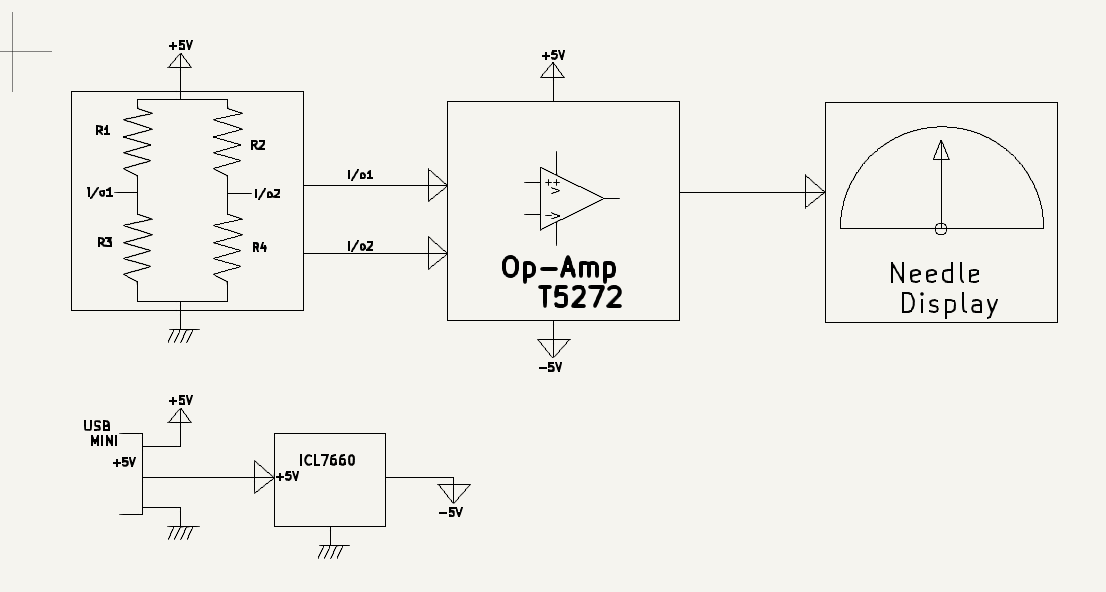
\includegraphics[width=0.7\linewidth]{images/Block_Diagram.png}
    \caption{Block Diagram}
    \label{fig:placeholder}
\end{figure}

\subsection{ Operational Overview}
\begin{itemize}
    \item Bridge Balancing
        Initially, the user adjusts two potentiometers (10 k\textohm coarse and 1 k\textohm fine) to balance the Wheatstone Bridge. This ensures that the voltage difference across the bridge output is zero, and the needle rests in the central (zero) position.
    \item Heating and Resistance Change
        When the resistor is heated using a hot air gun or soldering iron, its resistance either increases or decreases depending on its material and thermal behavior. This disturbs the balance of the bridge and creates a small differential voltage.
     \item Amplification   
        This differential voltage is fed into a differential amplifier built using a TS272 op-amp. The amplifier magnifies the voltage change by a factor of approximately 10×.
     \item Needle Deflection  
        The amplified voltage is sent to a mechanical pointer system (such as a modified meter), where the needle deflects left or right depending on the polarity and magnitude of the voltage. A leftward deflection suggests a decrease in resistance (NTC-like), while a rightward deflection suggests an increase (PTC-like).
    \item Dual Power Supply
        The op-amp requires a $\pm$5V supply. This is achieved by using a mini USB connector to provide $+5\,\mathrm{V}$, and an ICL7660 IC to generate the $-5\,\mathrm{V}$ rail.
\newpage
\section{Board Schematic}
\begin{figure}[H]
    \centering
    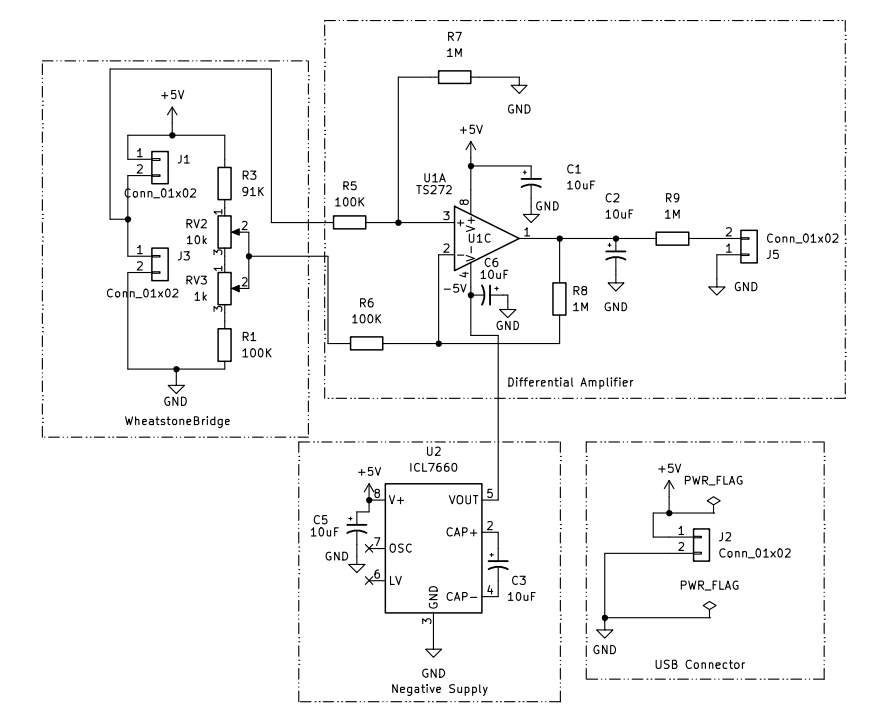
\includegraphics[width=1\linewidth]{images/schematic.png}
    \caption{PCB Schematic}
    \label{fig:placeholder}
\end{figure}

\newpage  
\section{Board Layout}
\begin{figure}[H]
    \centering
    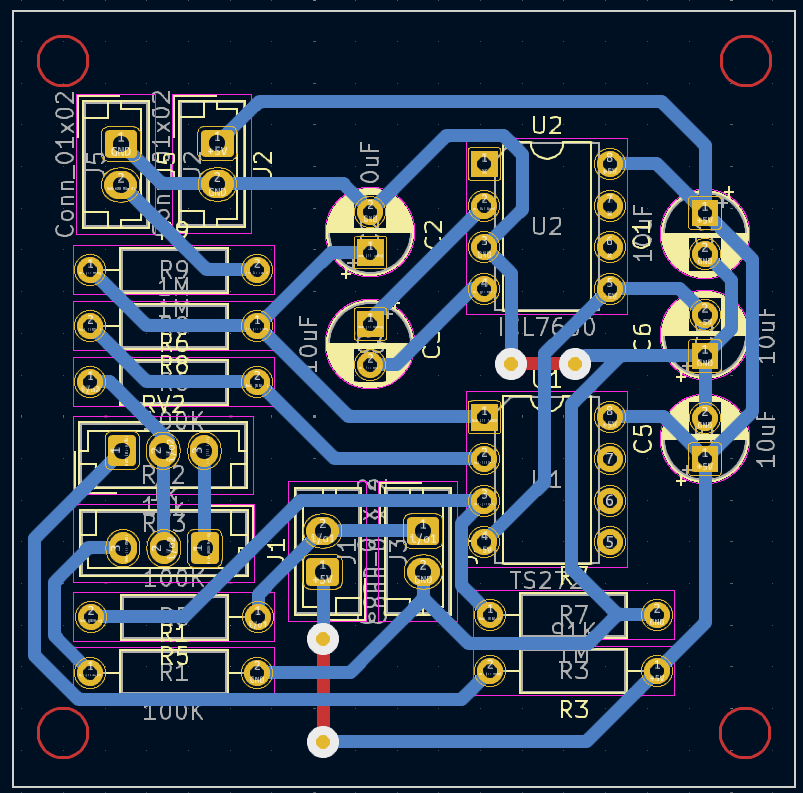
\includegraphics[width=0.8\linewidth]{images/board layout.png}
    \caption{PCB layout}
    \label{fig:placeholder}
\end{figure}
 \end{itemize}
\newpage

\newpage
\section{Bill of Material}
\begin{figure}[H]
    \centering
    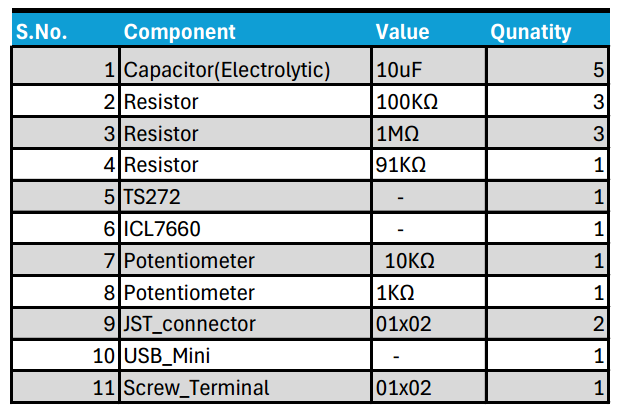
\includegraphics[width=1\linewidth]{images/Bill of Material.png}
    \caption{Bill of Materials}
    \label{fig:placeholder}
\end{figure}
\end{document}
